\documentclass{article}
\usepackage{amssymb}
\usepackage{amsmath}
\usepackage{float}
\usepackage{microtype}
\usepackage{tikz}

\newcommand \dP {\;\mathrm{d}\mathbb{P}}


\title{Probabilistic Modes of Convergence}
\author{William G Underwood}

\begin{document}

\maketitle

\section{Introduction}

In probability theory, we use several notions of `convergence' for
a sequence of random variables.
Some of these notions are stronger than others, so it is natural to ask
when one convergence implies another.
In the following definitions and results, we assume that $X$ and $(X_n)_{n \geq 1}$ are all
real-valued random variables on some complete probability space
$(\Omega, \mathcal{F}, \mathbb{P})$.


\section{Definitions}

Below are definitions for a few of the more
commonly-used modes of convergence.

\subsection*{Almost sure convergence ($a.s.$)}

$X_n \xrightarrow{a.s.} X$
if
$$\mathbb{P}(X_n \to X \text{ as } n \to \infty) = 1$$

\subsection*{Convergence in probability ($\mathbb{P}$)}

$X_n \xrightarrow{\mathbb{P}} X$
if for all $\epsilon > 0$,
as $n \to \infty$,
$$\mathbb{P}(|X_n - X| > \epsilon) \to 0$$

\subsection*{Convergence in distribution ($d$)}

$X_n \xrightarrow{d} X$
if whenever $\mathbb{P}(X \leq \,\boldsymbol{\cdot}\,)$ is continuous at $x$,
then as $n \to \infty$,
$$\mathbb{P}(X_n \leq x) \to \mathbb{P}(X \leq x)$$

\subsection*{Convergence in $L^p$, for $1 \leq p < \infty$}

$X_n \xrightarrow{L^p} X$
if as $n \to \infty$,
$$\mathbb{E}[|X_n - X|^p] \to 0$$

\subsection*{Convergence in $L^\infty$}

First define $\|X\|_\infty = \inf\{M: |X| \leq M \text{ almost surely}\}$.
Then $X_n \xrightarrow{L^\infty} X$
if as $n \to \infty$,
$$\|X_n - X\|_\infty \to 0$$

\subsection*{Notes on definitions}

Almost sure convergence is the natural measure-theoretic extension of the
notion of pointwise convergence of functions.
We simply require the convergence to occur at almost every point rather
than at every point.

Convergence in probability is (as we will see) weaker than this, and means that
with high probability, $(X_n)$ will not make large deviations from $X$.

Convergence in distribution is even weaker, and depends only on the
distributions of the random variables.
The random variables do not even need to be defined on the same probability space.

The $L^p$ spaces define a whole family of modes of convergence, with a larger value of $p$ giving
stronger convergence.
Convergence in $L^\infty$ is the same as uniform convergence almost everywhere.


\section{Results}

All of the results are summarised in Figure~\ref{fig:diagram}.
Arrows indicate strength of convergence.


\begin{figure}[H]
\centering
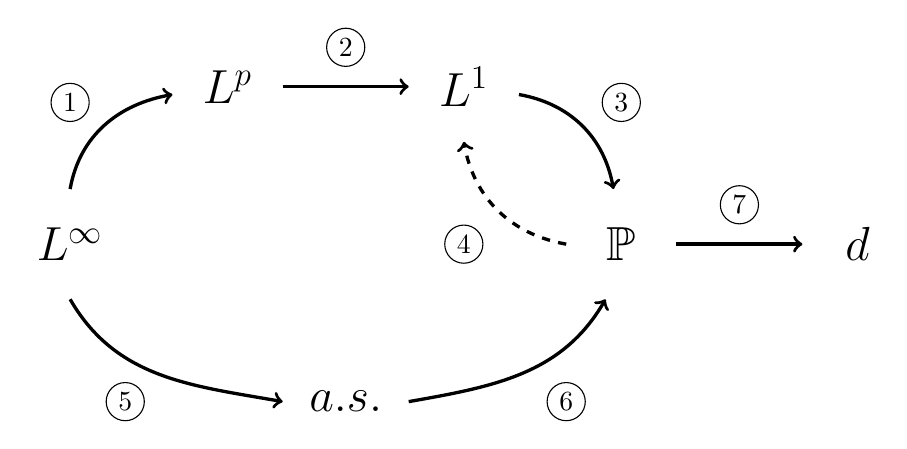
\begin{tikzpicture}

  % nodes
  \node at (0,0) {\LARGE $L^\infty$};
  \node at (2,2) {\LARGE $L^p$};
  \node at (5,2) {\LARGE $L^1$};
  \node at (7,0) {\LARGE $\mathbb{P}$};
  \node at (10,0) {\LARGE $d$};
  \node at (3.5,-2) {\LARGE $a.s.$};

  % arrows
  \draw [->, very thick] (0,0.7) to [out=80,in=190] (1.3,1.9);
  \draw [->, very thick] (2.7,2) -- (4.3,2);
  \draw [->, very thick] (5.7,1.9) to [out=-10,in=100] (6.9,0.7);
  \draw [->, very thick, dashed] (6.3,0) to [out=170,in=-80] (5,1.3);
  \draw [->, very thick] (7.7,0) -- (9.3,0);
  \draw [->, very thick] (0,-0.7) to [out=-60,in=170] (2.7,-2);
  \draw [->, very thick] (4.3,-2) to [out=10,in=-120] (6.8,-0.7);

  % labels
  \node[circle,draw,inner sep=2pt] at (0,1.8) {1};
  \node[circle,draw,inner sep=2pt] at (3.5,2.5) {2};
  \node[circle,draw,inner sep=2pt] at (7,1.8) {3};
  \node[circle,draw,inner sep=2pt] at (5,0) {4};
  \node[circle,draw,inner sep=2pt] at (0.7,-2) {5};
  \node[circle,draw,inner sep=2pt] at (6.3,-2) {6};
  \node[circle,draw,inner sep=2pt] at (8.5,0.5) {7};

\end{tikzpicture}
\caption{Modes of convergence}\label{fig:diagram}
\end{figure}


\section{Proofs}

A proof is given for each arrow in Figure~\ref{fig:diagram}.

\subsection*{1. $L^\infty$ convergence implies $L^p$ convergence}
\begin{align*}
  \mathbb{E}[|X_n - X|^p]
  &= \int_\Omega |X_n - X|^p \dP \\
  &\leq \|X_n - X\|_\infty^p \int_\Omega \dP \\
  &\to 0
\end{align*}


\subsection*{2. $L^p$ convergence implies $L^1$ convergence}
\begin{align*}
  \mathbb{E}[|X_n - X|]^p
  &\leq \mathbb{E}[|X_n - X|^p]
  & \text{(Jensen's inequality for $p \geq 1$)} \\
  &\to 0
\end{align*}

\subsection*{3. $L^1$ convergence implies convergence in probability}
\begin{align*}
  \mathbb{P}(|X_n - X| > \epsilon)
  &= \int_\Omega \mathbb{I}\{|X_n - X| > \epsilon\} \dP \\
  &\leq \int_\Omega \frac{1}{\epsilon} \, |X_n - X| \dP & \text{(Markov's inequality)} \\
  &\leq \frac{1}{\epsilon} \, \mathbb{E}[|X_n - X|] \\
  &\to 0
\end{align*}

\subsection*{4. Convergence in probability implies convergence in $L^1$,
in a uniformly integrable family}
Assuming $(X_n)$ is uniformly integrable; for any $\epsilon > 0$,
there is a $\delta > 0$ such that for
any $B \in \mathcal{F}$,
$$\mathbb{P}(B) < \delta \implies \int_\Omega |X_n - X| \, \mathbb{I}_B \dP < \frac{\epsilon}{2}$$
%
Also, $X_n \xrightarrow{\mathbb{P}} X$ so there is an $N \in \mathbb{N}$ such that
$$n \geq N \implies \mathbb{P}\left(|X_n - X| \geq \frac{\epsilon}{2}\right) < \delta$$
%
Putting these together:
\begin{align*}
  \mathbb{E}[|X_n - X|]
  &= \int_\Omega |X_n - X| \, \mathbb{I}\left\{|X_n - X| < \frac{\epsilon}{2}\right\} \dP \\
  &\qquad + \int_\Omega |X_n - X| \, \mathbb{I}\left\{|X_n - X| \geq \frac{\epsilon}{2}\right\} \dP \\
  &< \epsilon
\end{align*}



\subsection*{5. $L^\infty$ convergence implies almost sure convergence}
Since $\|X_n - X\|_\infty \to 0$;
for any $\epsilon>0$ there is an $N \in \mathbb{N}$ such that
$$n \geq N \implies \|X_n - X\|_\infty < \epsilon$$
%
So by the definition of $\|\cdot\|_\infty$,
\begin{align*}
  &\quad \,\, \mathbb{P}(|X_n - X| > \epsilon \text{ for some } n \geq N) \\
  &\leq \mathbb{P}(|X_n - X| > \|X_n - X\|_\infty \text{ for some } n \geq N) \\
  &= \mathbb{P}\Big(\bigcup_{n=1}^\infty \big\{|X_n - X| > \|X_n - X\|_\infty \big\} \Big) \\
  &\leq \sum_{n=1}^\infty \mathbb{P}\big(|X_n - X| > \|X_n - X\|_\infty \big) \\
  &= 0
\end{align*}

\subsection*{6. Almost sure convergence implies convergence in probability}
Fix $\epsilon$ and let
$A_N = \{|X_n - X| < \epsilon \text{ for all } n \geq N\}$.
Note that $A_N$ increases to
$$\bigcup_{N=1}^\infty A_N = \{|X_n - X| < \epsilon \text{ eventually}\}
\supseteq \{X_n \to X\}$$
%
Therefore
\begin{align*}
  \mathbb{P}(|X_N - X| < \epsilon)
  &\geq \mathbb{P}(A_N) \\
  &\to \mathbb{P}\Big(\bigcup_{N=1}^\infty A_N\Big) \\
  &\geq \mathbb{P}(X_n \to X) \\
  &= 1
\end{align*}

\subsection*{7. Convergence in probability implies convergence in distribution}
Take $x$ a continuity point of $\mathbb{P}(X \leq \,\boldsymbol{\cdot}\,)$, and
fix $\epsilon > 0$.
\begin{align*}
  \mathbb{P}(X_n \leq x)
  &\leq \mathbb{P}(X \leq x+\epsilon) + \mathbb{P}(|X_n - X| > \epsilon) \\
  &\to \mathbb{P}(X \leq x+\epsilon) \qquad \text{as } n \to \infty
\end{align*}
%
Similarly
\begin{align*}
  \mathbb{P}(X_n \leq x)
  &\geq \mathbb{P}(X \leq x-\epsilon) - \mathbb{P}(|X_n - X| > \epsilon) \\
  &\to \mathbb{P}(X \leq x-\epsilon) \qquad \text{as } n \to \infty
\end{align*}
%
So $\mathbb{P}(X_n \leq x) \to \mathbb{P}(X \leq x)$, by continuity at $x$.



\end{document}
